% ═══════════════════════════════════════════════════════════════════════════════
%  Capítulo 1 — Introducción
%  TFM: Detección de Aeronaves No Tripuladas mediante Señales de RF y
%       Redes Neuronales de Valor Complejo en Entornos de Baja SNR
% ═══════════════════════════════════════════════════════════════════════════════

\chapter{Introducción}
\label{cap:introduccion}

% ───────────────────────────────────────────────────────────────────────────────
\section{Contexto y motivación}
\label{sec:contexto}
% ───────────────────────────────────────────────────────────────────────────────

\lettrine{E}{l} rápido desarrollo de los vehículos aéreos no tripulados, comunmente denominados \gls{uav}, ha dado lugar a una transformación directa y muy profunda del espacio aéreo de baja altitud. Desde su origen como plataformas exclusivamente militares de reconocimiento y ataque de precisión, los \gls{uav} han evolucionado hasta convertirse en herramientas de uso cotidiano tanto en aplicaciones civiles, como fotografía aérea, cartografía, agricultura de precisión o reparto de mercancías, como en contextos de seguridad y defensa nacional. Según estimaciones del mercado global, el número de \gls{uav} civiles en operación superó los 800\,000 en Europa en 2024, con proyecciones que anticipan una triplicación para el año 2030 \cite{sesar_outlook_2016}.

Esta proliferación masiva conlleva riesgos cuya gestión eficaz constituye uno de los desafíos tecnológicos más relevantes de la década presente. Los incidentes en aeropuertos internacionales, como el cierre del Aeropuerto de Gatwick (que ocupa el segundo lugar en superficie total y movimiento de parajeros entre todos los aeropuertos de Londres) en diciembre de 2018 que afectó a más de 140\,000 pasajeros \cite{dft_taking_flight_2019}, ilustran la dimensión operativa del problema en entornos civiles. En el ámbito militar, durante los conflictos armados más recientes se ha generalizado el empleo de drones para operaciones de reconocimiento, identificación de objetivos y como vectores de ataque. El ejemplo más claro es la actual guerra en Ucrania, la cual ha evidenciado el uso sistemático de plataformas comerciales de bajo coste para misiones de vigilancia y guerra electrónica, así como su adaptación para el lanzamiento de cargas explosivas y su empleo en ataques de impacto directo, redefiniendo así las doctrinas de defensa terrestre contemporáneas \cite{lacy_machine_2024}. En este contexto, la detección fiable de drones se ha convertido en una capacidad estratégica de primer orden.

Los sistemas de contención de \gls{uav}, conocidos en la literatura como sistemas \gls{c-uas} o anti-dron, abarcan un espectro muy amplio de distintas tecnologías. Los enfoques basados en señales de radiofrecuencia (RF) han emergido como los más adecuados para su despliegue en entornos críticos debido a su velocidad de respuesta, robustez y capacidad de detección sin necesidad de línea de visión directa y desde una distancia sustancialmente mayor en comparación con otras modalidades (como radar activo, sensores electroópticos o detección acústica), que presentan limitaciones operativas fundamentales \cite{ezuma_micro-uav_2019, ezuma_detection_2020}. Sin embargo, según diversos autores, los enfoques convencionales de detección por RF exhiben una degradación severa del rendimiento cuando la \gls{snr} de la señal objetivo desciende por debajo de los $0$\,dB, umbral que caracteriza los escenarios de operación encubierta, vuelo a larga distancia o entornos con mucha interferencia \cite{ezuma_detection_2020, flak_rf_2023, ozturk_rf-based_2021}.

El presente Trabajo Fin de Máster aborda precisamente este reto: desarrollar y evaluar un sistema de detección de \gls{uav} basado en el análisis de señales de radiofrecuencia en bruto (como señales en fase y cuadratura, I/Q), mediante técnicas de \textit{machine learning} y \textit{deep learning}, con énfasis específico en la robustez bajo condiciones de baja \gls{snr}. Esta investigación propone y evalúa una familia de arquitecturas de redes neuronales de valor complejo (\gls{cv-cnn}) que operan directamente sobre la señal I/Q.

% ───────────────────────────────────────────────────────────────────────────────
\section{Situación actual: implicaciones en defensa, privacidad y seguridad}
\label{sec:situacion_actual}
% ───────────────────────────────────────────────────────────────────────────────

Como se ha comentado anteriormente, el uso a gran escala de drones de bajo coste ha generado un conjunto de amenazas transversales que trascienden los límites del ámbito militar y afectan a la seguridad pública, la privacidad y la protección de infraestructuras críticas. A continuación se describen los casos de riesgo más relevantes identificados en la literatura reciente.

\paragraph{Vigilancia no autorizada y vulneración de la privacidad.}\mbox{}\\[0.5em]
Los drones equipados con cámaras de alta resolución y sensores térmicos constituyen una herramienta de vigilancia encubierta de bajo coste y difícil detección. Incidentes documentados incluyen el sobrevuelo sistemático de instalaciones militares en varios países de la OTAN, la captación de imágenes sobre centros penitenciarios o la monitorización de eventos de masas sin autorización administrativa. El marco regulatorio europeo, establecido por el Reglamento (UE) 2019/945 de la Agencia Europea de Seguridad Aérea (EASA), clasifica los \gls{uav} según su riesgo operacional e impone obligaciones de registro e identificación electrónica a distancia; sin embargo, la brecha entre la norma y la capacidad tecnológica de verificación sigue siendo significativa \cite{ezuma_detection_2020}.

\paragraph{Uso como vector de ataque.}\mbox{}\\[0.5em] 
El empleo de drones como vectores de ataque directo, incluyendo tácticas de ataque directo o \textit{kamikazes}, se ha consolidado como una táctica recurrente en conflictos modernos. Organismos como el Departamento de Defensa de los Estados Unidos y el Estado Mayor Conjunto de las Fuerzas Armadas Españolas han identificado el aumento de enjambres de \gls{uav}s como una de las amenazas emergentes de mayor prioridad para las próximas décadas \cite{dod_cuas_2021}. Los ataques mediante enjambres de drones comerciales, coordinados mediante protocolos de comunicación distribuidos, son capaces de saturar los sistemas de defensa convencionales diseñados principalmente para tratar amenazas individuales, desbordando su capacidad operativa simultánea.

\paragraph{Perturbación de infraestructuras críticas.}\mbox{}\\[0.5em] 
Los aeropuertos, las plantas nucleares, los centros de datos y los sistemas de generación eléctrica constituyen algunos objetivos susceptibles a la perturbación inducida por estos dispositivos. La proximidad de un \gls{uav} a la trayectoria de aterrizaje de una aeronave comercial puede derivar en colisión con motores o superficies de control, con consecuencias potencialmente catastróficas. El Aeropuerto Heathrow de Londres registró 93 incidentes de acercamientos no autorizados de drones solo en 2023, cifra que demuestra la magnitud del problema en el caso de entornos aeroportuarios concurridos \cite{gluge_robust_2024}.

\paragraph{Marco regulatorio y limitaciones vigentes.}\mbox{}\\[0.5em] 
La respuesta regulatoria a esta problemática ha avanzado de forma desigual a escala global. La EASA introdujo en enero de 2021 un marco de identificación remota obligatoria que exige la emisión periódica de un identificador único por parte de todo drones en vuelo \cite{easa_remoteid_2021}. Sin embargo, este mecanismo es trivialmente eludible por operadores que desactiven el módulo correspondiente, y no proporciona ninguna capacidad de detección autónoma por parte de los sistemas de seguridad. Esta limitación intrínseca del enfoque regulatorio refuerza la necesidad de sistemas de detección tecnológicamente robustos e independientes de la colaboración del operador del dispositivo.

El análisis detallado de las tecnologías actuales para solventar este tipo de problemas mencionados anteriormente, y las principales plataformas comerciales y militares actuales se aborda en el Capítulo~\ref{cap:EstadoDelArte}.

% ───────────────────────────────────────────────────────────────────────────────
\section{Limitaciones fundamentales de los enfoques basados en RF}
\label{sec:limitaciones}
% ───────────────────────────────────────────────────────────────────────────────

A pesar de los avances reseñados, los sistemas C-UAS basados en radiofrecuencia presentan un conjunto de limitaciones estructurales que condicionan su eficacia en escenarios operativos reales. Su constituye el punto de partida que motiva la investigación llevada a cabo en este trabajo.

\paragraph{Degradación del rendimiento en baja SNR.}\mbox{}\\[0.5em]
Los sistemas basados en análisis RF, tal y como se ha expuesto anteriormente, exhiben una pérdida de rendimiento muy notable cuando la \gls{snr} de la señal objetivo desciende por debajo de valores positivos. En este régimen, los detectores de energía convencionales no consiguen distinguir la señal del \gls{uav} del ruido de fondo electromagnético, en particular cuando coexisten fuentes de interferencia como redes Wi-Fi, dispositivos Bluetooth y señales \gls{awgn}. Esta limitación es especialmente pronunciada cuando el \gls{uav} opera a distancias superiores a los 300\,m o en entornos urbanos con alta densidad espectral de interferentes \cite{gluge_robust_2024, lacy_machine_2024}.

\paragraph{Proliferación de enjambres y coordinación distribuida.}\mbox{}\\[0.5em]
Las arquitecturas de ataque mediante enjambres de \gls{uav}, que distribuyen la funcionalidad entre múltiples unidades de bajo coste en lugar de concentrarla en una plataforma singular, representan un vector de amenaza cualitativamente distinto al que los sistemas C-UAS actuales no se encuentran optimizados para responder. La coordinación entre unidades puede realizarse mediante protocolos de comunicación de malla de baja potencia, en frecuencias fuera de las bandas convencionales de supervisión, o incluso de forma completamente offline mediante algoritmos de enjambre predeterminados. La respuesta eficaz a esta amenaza requiere sistemas capaces de procesar múltiples señales simultáneas con tiempos de latencia reducidos.

\paragraph{Congestión espectral y falsos positivos.}\mbox{}\\[0.5em]
En entornos urbanos densamente poblados, el espectro electromagnético en las bandas de 2,4\,GHz y 5,8\,GHz está saturado por dispositivos Wi-Fi, Bluetooth, teléfonos inteligentes y otros sistemas que emiten señales espectralmente similares a las de los protocolos de control de \gls{uav}. Los sistemas C-UAS convencionales presentan tasas de falsos positivos elevadas en estos entornos, lo que los hace operativamente inviables para su despliegue en zonas metropolitanas sin intervención humana continua. La tasa de falsas alarmas es un parámetro crítico en las especificaciones militares de sistemas de defensa, dado que la neutralización de un objetivo legítimamente identificado como amenaza, como una aeronave comercial, puede tener consecuencias catastróflicas.

\paragraph{Limitaciones de generalización entre plataformas.}\mbox{}\\[0.5em] 
Los sistemas basados en bases de datos de firmas espectrales estáticas requieren actualización continua ante la aparición de nuevos modelos de \gls{uav}, tarea que resulta inviable a la escala de la proliferación actual del mercado. Los enfoques de aprendizaje automático que aprenden representaciones genéricas de las señales, en lugar de depender de firmas preprogramadas, ofrecen una mayor robustez frente a plataformas desconocidas, aunque su eficacia disminuye notablemente cuando la \gls{snr} disponible no permite la extracción de rasgos discriminativos fiables \cite{ezuma_micro-uav_2019}.

% ───────────────────────────────────────────────────────────────────────────────
\section{Objetivos y contribuciones del trabajo}
\label{sec:objetivos}
% ───────────────────────────────────────────────────────────────────────────────

A la vista de las limitaciones identificadas, el presente trabajo se propone avanzar
en el estado del arte de la detección de \gls{uav} mediante señales RF en condiciones
adversas de \gls{snr}. La pregunta de investigación central que guía el trabajo es la
siguiente:

\begin{quote}
\textit{¿Es posible diseñar un sistema de detección de \gls{uav} basado en señales RF
en bruto que mantenga un rendimiento de clasificación aceptable, superior al
80\,\% de exactitud global, en escenarios con SNR inferior a $-6$\,dB, en
presencia simultánea de interferencias Wi-Fi y Bluetooth?}
\end{quote}

Para dar respuesta a esta pregunta, el trabajo realiza las siguientes contribuciones
principales:

\begin{enumerate}

  \item \textbf{Diseño y evaluación de una familia de arquitecturas \gls{cv-cnn} para
  señales IQ.} Se proponen tres variantes arquitectónicas, denominadas
  \textit{SingleStream-CVCNN}, \textit{DualStream-SlidingWindow} y
  \textit{DualStream-DynamicSlidingWindow}, que operan directamente sobre señales
  IQ en bruto mediante convoluciones complejas de Wirtinger, preservando la
  información de fase de la señal.

  \item \textbf{Integración de un detector energético adaptativo CFAR con extracción
  de características físicas.} Se desarrolla un detector basado en la entropía de
  Shannon sobre la \gls{stft} de la señal, configurado con un mecanismo adaptativo de
  umbral tipo \gls{cfar}, cuyas salidas se utilizan para guiar la segmentación temporal
  de la señal y extraer un vector de ocho características físicas que complementa
  la representación neuronal.

  \item \textbf{Desarrollo y validación de un esquema de pseudo-etiquetado mediante
  oráculo físico.} Se propone un sistema de etiquetado automático de ráfagas
  individuales a bajo \gls{snr} basado en la coherencia temporal de las duraciones de
  los saltos \gls{fhss}, que permite ampliar el conjunto de entrenamiento sin
  necesidad de etiquetado manual en el dominio de baja \gls{snr}.

  \item \textbf{Evaluación experimental exhaustiva sobre el conjunto de datos
  NoisyUAV.} Se reportan métricas de rendimiento desagregadas por nivel de \gls{snr},
  por modelo de emisor RF y por modalidad de interferencia, sobre el conjunto de
  datos NoisyUAV, que constituye el repositorio de señales RF de \gls{uav} con mayor
  diversidad de condiciones electromagnéticas adversas disponible públicamente.

\end{enumerate}

Para facilitar la comprensión global de la solución propuesta, la Figura~\ref{fig:esquema_general} ilustra de manera simplificada la arquitectura de detección diseñada en este trabajo, mostrando el flujo de la señal desde la captura RF hasta la decisión del clasificador.

\begin{figure}[H]
    \centering
    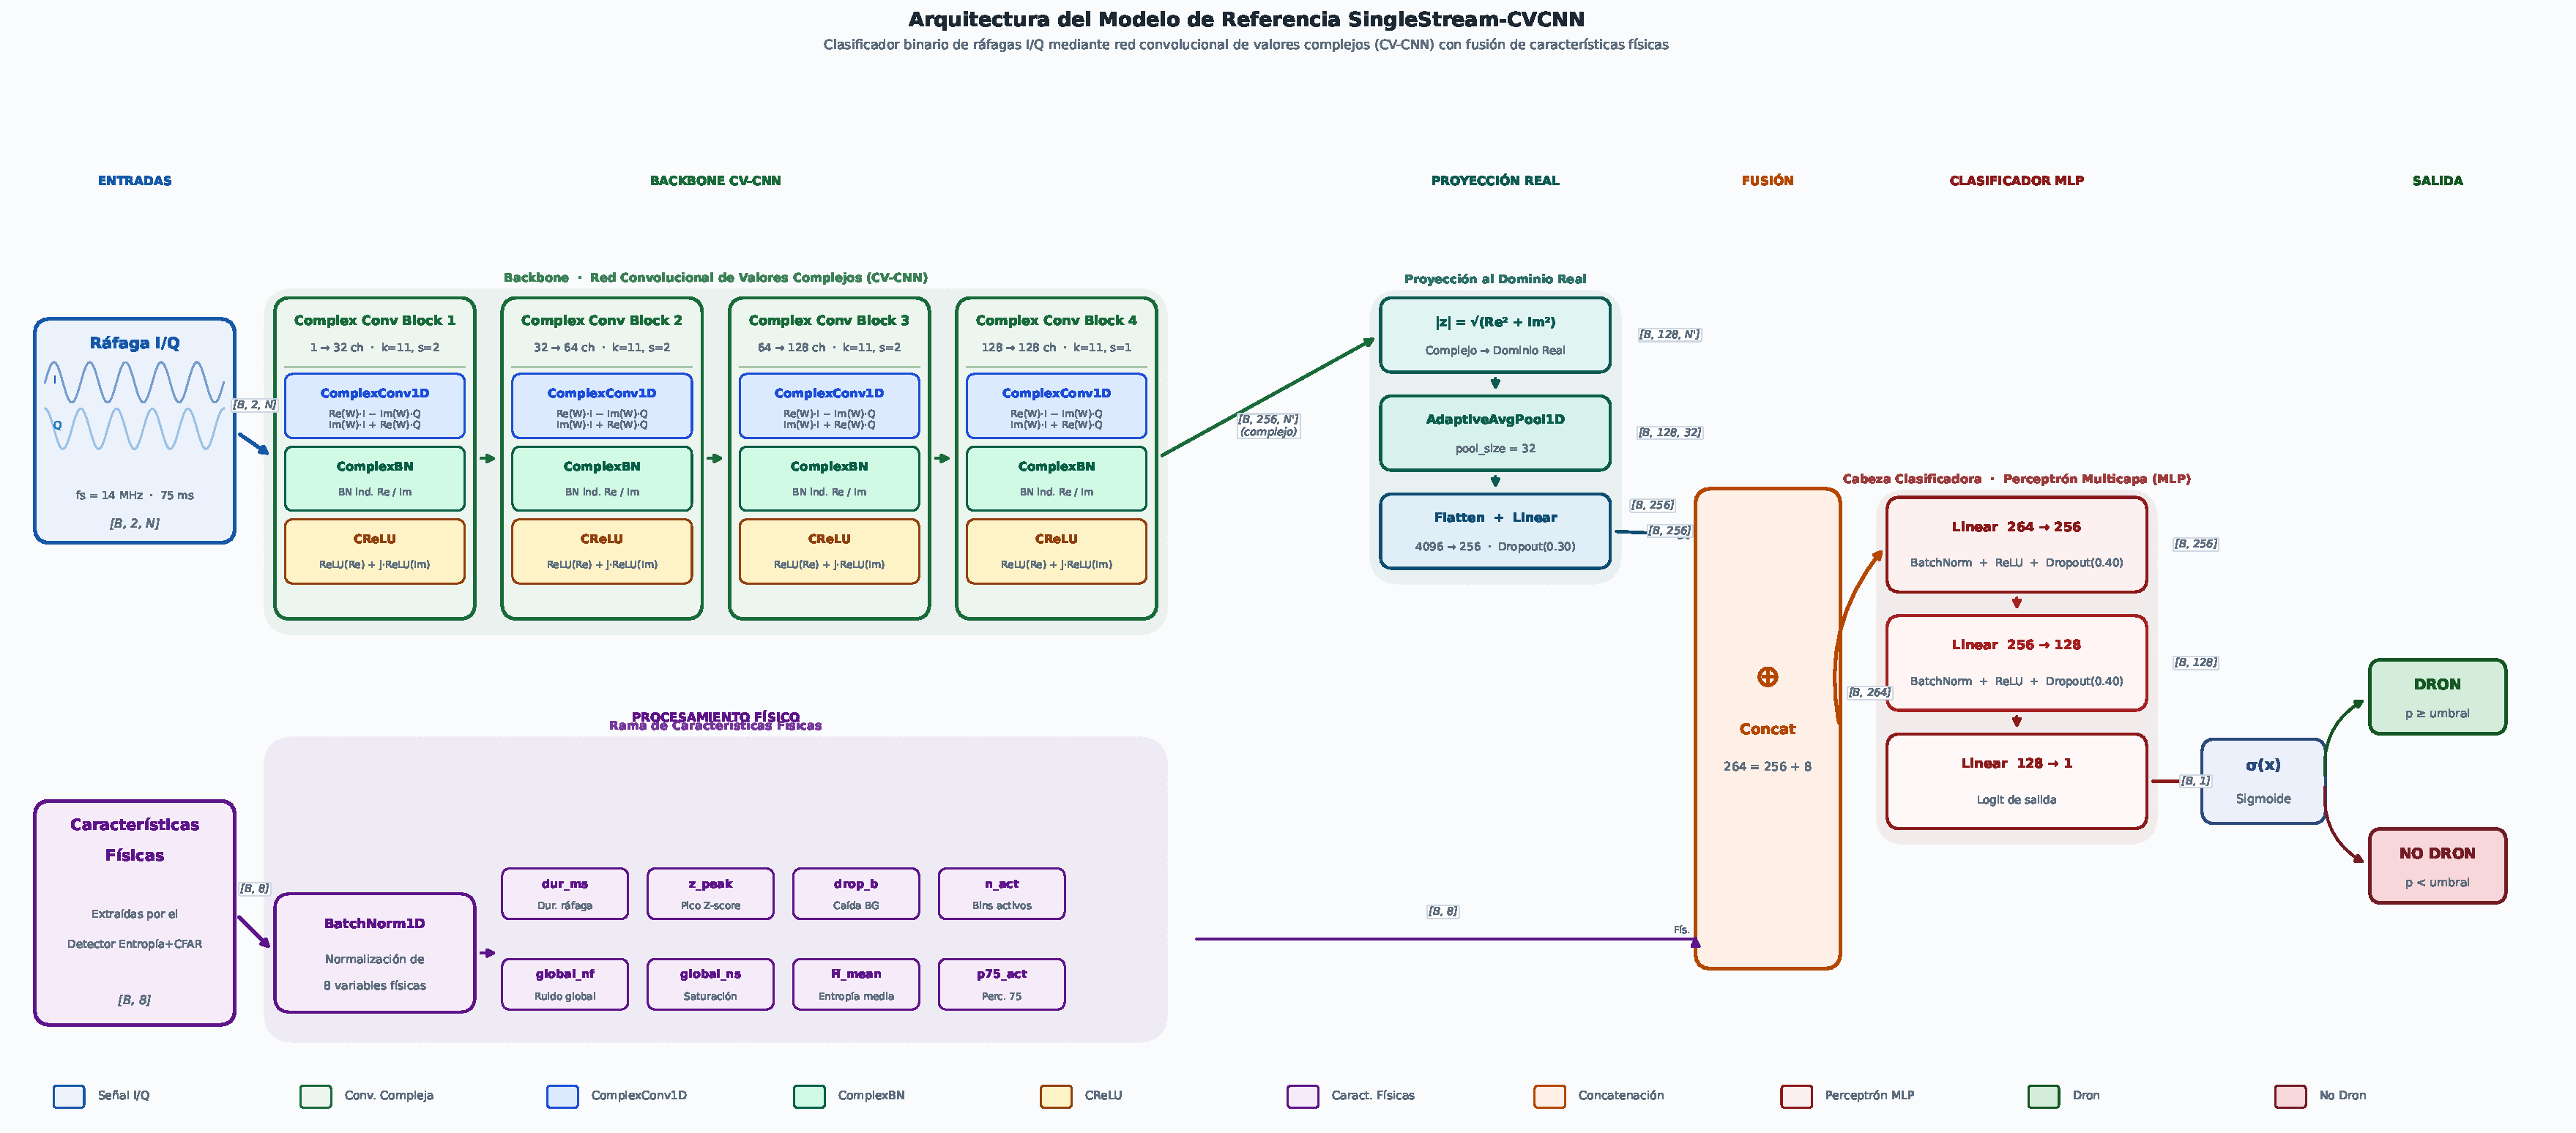
\includegraphics[width=0.85\linewidth]{../figuras_arquitectura/singlestream_architecture.pdf}
    \caption{Esquema general simplificado de la arquitectura de detección de \gls{uav} propuesta basada en redes neuronales de valor complejo y extracción de características físicas.}
    \label{fig:esquema_general}
\end{figure}


Para facilitar la comprensión global de la solución propuesta, la Figura~\ref{fig:esquema_general} ilustra de manera simplificada la arquitectura de detección diseñada en este trabajo, mostrando el flujo de la señal desde la captura RF hasta la decisión del clasificador.

\begin{figure}[H]
    \centering
    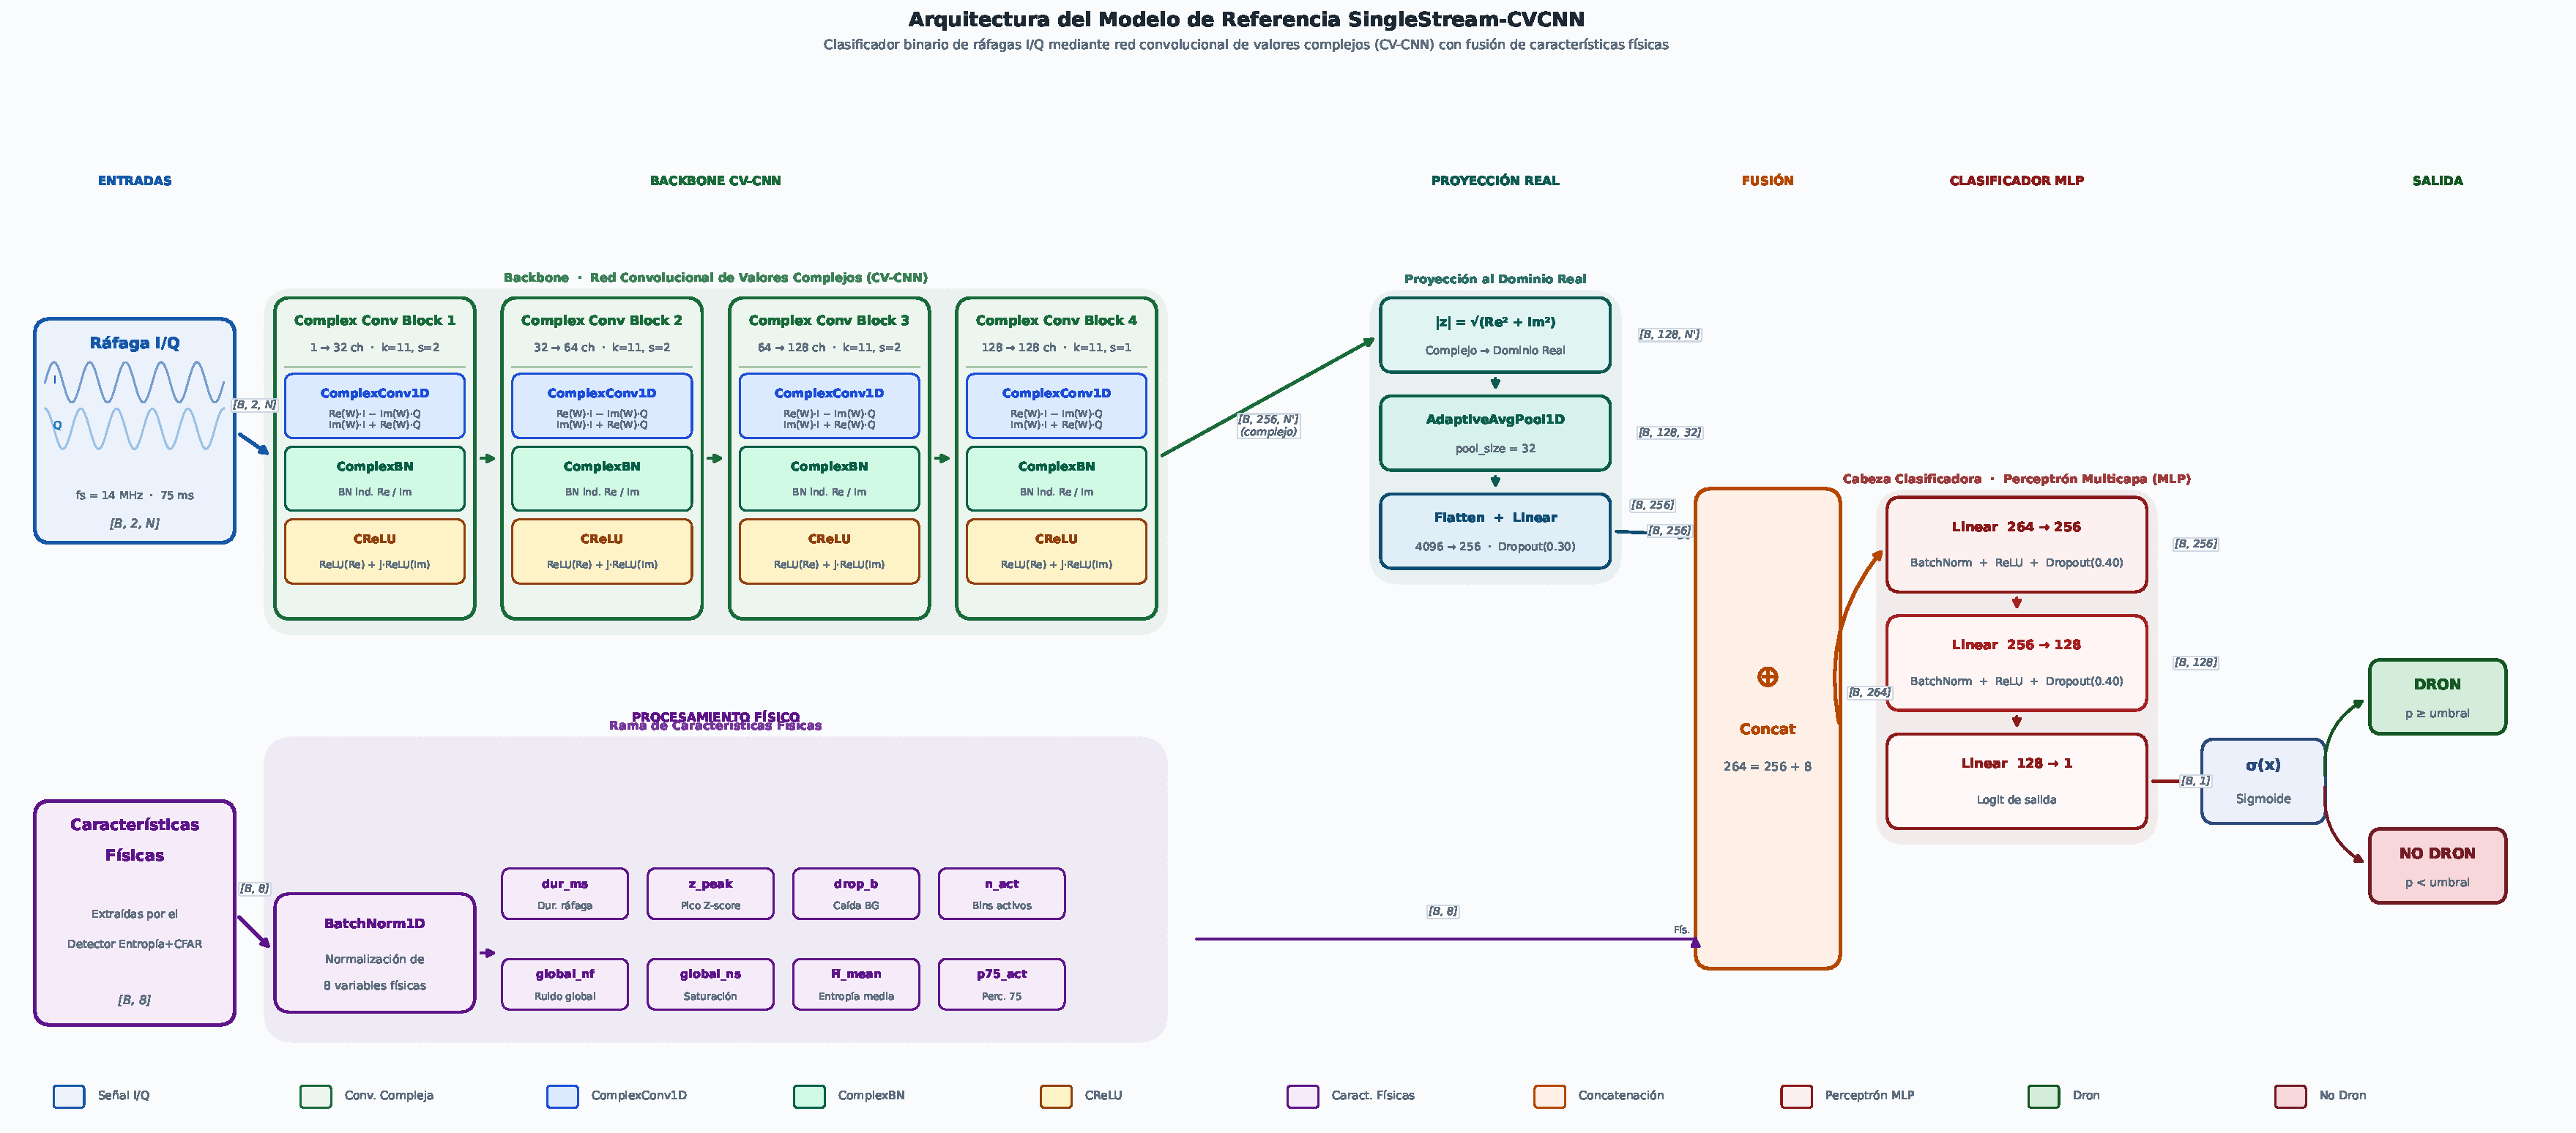
\includegraphics[width=0.85\linewidth]{../figuras_arquitectura/singlestream_architecture.pdf}
    \caption{Esquema general simplificado de la arquitectura de detección de \gls{uav} propuesta basada en redes neuronales de valor complejo y extracción de características físicas.}
    \label{fig:esquema_general}
\end{figure}


% ───────────────────────────────────────────────────────────────────────────────
\section{Estructura del documento}
\label{sec:estructura}
% ───────────────────────────────────────────────────────────────────────────────

El presente documento se organiza en seis capítulos. El Capítulo~\ref{cap:EstadoDelArte}
revisa el estado del arte en detección de \gls{uav} mediante señales RF, con énfasis
en los enfoques basados en aprendizaje automático y en los conjuntos de datos
públicos disponibles para su evaluación. El Capítulo~\ref{cap:MarcoTeorico} describe
el entorno experimental, el conjunto de datos NoisyUAV y el protocolo de evaluación
empleado. El Capítulo~\ref{cap:Arquitectura} detalla las arquitecturas propuestas,
su fundamentación teórica y las decisiones de diseño adoptadas. El
Capítulo~\ref{cap:ResultadosDiscusion} presenta los resultados experimentales y
discute su significado en relación con el estado del arte. Finalmente, el
Capítulo~\ref{cap:Conclusiones} resume las contribuciones del trabajo y propone
líneas de investigación futura.
